\subsection{Decision 6: Database scope and organization}

\subsection*{Status}
Review.

\subsection*{Architectural Summary}


\subsection*{Context}
We need to answer the following questions:
\begin{itemize}
\item Which info do we keep in the database? 
\item Do we need one or many databases?
\item How do we handle data protection?
\item How do we handle data update from tycoons/station management? (maybe for another decision?)
\end{itemize}

\subsection*{Concern}
We need to keep some information available from our system, but security of the data (especially payment and account data) is crucial for the government and for the passengers concerns.

\subsubsection*{User stories}
The following user stories are particularly relevant to the decision on the database scope, emphasizing the need for comprehensive management of subscriptions, security, and system integration:

\begin{itemize}[noitemsep]
    \item \textbf{User Story 1:} As a frequent traveler, I want to subscribe to a comprehensive monthly pass that includes all three networks so that I can save money on my regular commutes.
    
    \item \textbf{User Story 2:} As a passenger, I want to be able to check the balance of my multi-network travel card online so that I can easily manage my travel expenses.
    
    \item \textbf{User Story 3:} As a passenger with a subscription, I want to receive automatic notifications about my subscription renewal and any discounts or promotions available so that I can take advantage of cost savings. 
    
    \item \textbf{User Story 4:} As a tech-savvy passenger, I want to use a mobile app to manage my subscriptions, make payments, and receive digital tickets so that I can have a paperless and convenient travel experience. 
    
    \item \textbf{User Story 5:} As a passenger interested in sustainability, I want the system to track my travel carbon footprint and offer carbon offset options so that I can make environmentally responsible travel choices.
    
    \item \textbf{User Story 6:} As a passenger with mobility challenges, I want the payment system to provide information on accessible services and allow for easy purchase of accessible seating across all networks so that I can travel comfortably and safely.
    
    \item \textbf{User Story 16:} As a passenger, I want to be able to purchase a single ticket that allows me to travel across all train networks so that I can travel seamlessly without needing to buy separate tickets for each tycoon's network.
    
    \item \textbf{User Story 18:} As a government regulator, I want the payment system to adhere to data protection and financial transaction security standards so that passengers' personal and financial information is secure.
    
    \item \textbf{User Story 23:} As a tycoon, I want the payment system to integrate with my existing infrastructure with minimal disruption so that I can maintain high service levels during the transition.
    \item 
    \item \textbf{User Story 27:} As a network maintenance planner, I want the payment system to integrate with maintenance scheduling tools so that I can plan work with minimal disruption to the train service and revenue.
\end{itemize}

\subsection*{Option 1: Querying modules or external parties should know as little as possible}
We try to have one database for each important set of information that the system needs to know.
We try to stick to the Separation of Concerns principle, so that each module only has access to the data it scricly needs to operate.
We divide the following:
\begin{itemize}
    \item A database containing the timetable, the prices of seats and the bookings.
    \item A database containing the optimized routes cached after being calculated by the Routes Optimization Module.
    \item A database containing info about the accounts and their subscriptions. 
    \item A database recording payments that have been done, which should be accessed in case for example of complaints. 
\end{itemize}
\begin{figure}[ht]
    \centering
    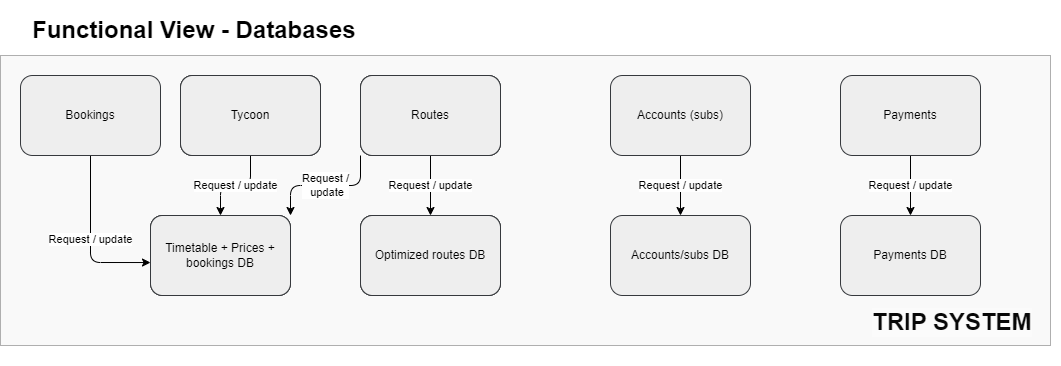
\includegraphics[width=\textwidth]{drawings/views_draft2/functional_view databases.png}
    \caption{Division of databases and their interaction with modules or stakeholders.}
    \label{fig:databases_view}
\end{figure}

\subsubsection*{Pros}
\begin{itemize}[noitemsep]
    \item \textbf{Enhanced Security} (Data Protection, Privacy): By segregating data across multiple databases, sensitive information is better protected, and access can be tightly controlled on a need-to-know basis.
    \item \textbf{Specialized Optimization} (Performance, Efficiency): Dedicated databases allow for optimization specific to their function, such as faster queries for timetable and booking data versus complex route optimization calculations.
\end{itemize}

\subsubsection*{Cons}
\begin{itemize}[noitemsep]
    \item \textbf{Increased Maintenance Overhead} (Maintainability, Complexity): Managing multiple databases adds complexity to the system's architecture, requiring more resources for maintenance and potentially higher costs.
    \item \textbf{Data Synchronization Challenges} (Reliability, Consistency): Ensuring data consistency across different databases can be challenging, especially in real-time, and may affect the system's overall reliability.
\end{itemize}

\subsection*{Option 2: Unified Centralized Database System}

This option proposes a centralized database architecture that consolidates all necessary information into a single, unified database system. It incorporates robust access control layers to manage data access based on module or user roles, ensuring that each part of the system accesses only the data it needs for operation. This model simplifies data management, enhances security through centralized control mechanisms, and facilitates easier updates and integrations. This model can be improved with having accounts database as a separate component, and keeping the rest of the databases central. In this way accounts data will be secure, and the rest of the systems will access accounts data anonymously via ids. Manage permissions for eacsh tycoon, on which info they can access (they shouldn't be able to connect name to bank account). In this way we can keep everything in the same place, but each tycoon api will have specificed access protocols. Tycoons can only update timetables and prices.

We can keep bookings data a DaaS, since it needs to be updated regularly and concurrently. Rest can be a server based database. Since we can cache routes we don't want cloud services for these. 

\subsubsection*{Pros}
\begin{itemize}[noitemsep]
    \item \textbf{Simplified Data Management} (Maintainability, Efficiency): Centralizing data storage simplifies the architecture by reducing the number of systems to manage, making it easier to maintain and update the database.
    \item \textbf{Improved Data Consistency} (Reliability, Integrity): A unified database ensures that all modules access the most current and consistent data, reducing the risk of discrepancies and errors.
    \item \textbf{Enhanced Integration Capability} (Scalability, Interoperability): With all data in one place, integrating new features, modules, or external systems becomes more straightforward, promoting scalability and interoperability.
\end{itemize}

\subsubsection*{Cons}
\begin{itemize}[noitemsep]
    \item \textbf{Risk of a Single Point of Failure} (Reliability, Availability): Centralizing data creates a single point of failure, which could potentially lead to system-wide outages affecting all functionalities if the database goes down.
    \item \textbf{Scalability Concerns} (Performance, Scalability): As the system grows, a centralized database might struggle with performance issues due to the increasing volume of data and concurrent access requests.
    \item \textbf{Complexity in Ensuring Data Protection} (Security, Privacy): Protecting a large, centralized repository of sensitive information poses significant challenges, requiring robust security measures to prevent unauthorized access and data breaches.
\end{itemize}

\subsection*{Option 3: Database per tycoon or not}

\subsubsection*{Pros}
\begin{itemize}[noitemsep]
    \item \textbf{Tycoon specific features} 
    \item \textbf{Tycoon access permissions are automatically managed} 
\end{itemize}

\subsubsection*{Cons}
\begin{itemize}[noitemsep]
    \item \textbf{Hard to manage the database} 
    \item \textbf{Shared data is potentially doubled} 
\end{itemize}

\subsection*{Option 4: Hybrid cloud storage}
Crucial data stored in cloud (timetables, and prices and bookings). Non-crucial data (accounts, payments) gets stored in non-cloud database one per tycoon, such that they can only access their own customer data.

\subsubsection*{Pros}
\begin{itemize}[noitemsep]
    \item \textbf{Tycoon specific access for accounts data} 
    \item \textbf{Secure and qucik access to data crucial data} 
    \item \textbf{Cheap storage for non-crucial data} 
\end{itemize}

\subsubsection*{Cons}
\begin{itemize}[noitemsep]
    \item \textbf{Can get expensive} 
    \item \textbf{Implementation of two different database types and their interactions setup}
\end{itemize}

\subsection*{Decision}
We choose Hybrid cloud storage System, increased Availability which is important for event 2 which requirees less stringent Maintainability and cost requirements. Cloud increased cost and interaction between databases increase Maintainability compared to single database.
\subsection*{Consequences}
\textbf{Positive Consequences:}
\begin{itemize}
    \item \textbf{database as a service}: Single point of failure is reduced, scalable.
    \item \textbf{}: Single point of failure is reduced, scalable.
\end{itemize}
\textbf{Negative Consequences:}
\begin{itemize}
    \item \textbf{Tycoon permission management} : More complextiy, we need to restrict access for each tycoon.
    \item \textbf{Single point of failure} : If database fails, everything fails.(bad for availablity)[maybe a solution is backup database].
    \item \textbf{database as a service}: Expensive.
\end{itemize}